\documentclass[12pt]{article}
\usepackage{inputenc}
\usepackage[left=3.5cm, right=2cm,
top=2cm, bottom=2cm]{geometry}
\usepackage{indentfirst}
\setlength{\parindent}{1cm}
\setlength{\parskip}{2pt}
\usepackage{blindtext}
\usepackage{graphicx}
\usepackage{wrapfig}
\usepackage{transparent}

\usepackage{fancyhdr}
\pagestyle{fancy}
\fancyhf{}%lệnh này dùng để xóa mặc định
\lhead{\LaTeX\ Basics}
\rfoot{Trang \thepage}
\renewcommand{\headrulewidth}{1pt}
\renewcommand{\footrulewidth}{1pt}

%\renewcommand{\thefigure}{\footnotesize Figure \arabic{figure}}

\title{\LARGE\bf The heat is on: from the Arctic to Africa, wildlife is being hit hard by climate chaos}
\author{- The Guardian -}
\date{\today}
\usepackage{enumerate}
\renewcommand{\labelenumi}{\roman{enumi}}
\renewcommand{\labelenumii}{$\star$}
\begin{document}
Team works skill are necessary as our field involves carrying on big projects. Team working is one way to perfect ourselves through learning from others . 
 These team work skills are: 
 \begin{enumerate}
     \item Team building skill: create a group of peoople with regular interaction and together they achieve a goal.
     \item Dominant skills: is knowing how to achive efficiency like aiming a target, clearly seperating individual work, communicating, etc, ... Some of them are very important such as:
      \begin{enumerate}
         \item Communication: Well-interacted with your teammates to create friendly working environment and understand among members to gain efficiency.
         \item Conflict resolution: seeing through the conflict and using communication to solve.
         \item Hold up meetings: make a plan, step by step follow, using visual supporting; figures, maps, powerpoint,... 
     \end{enumerate}
\end{enumerate}
\newpage
\begin{center}
\begin{minipage}{0.8\textwidth}
\small\bf Global heating affects fertility, immunity and behaviour – often with lethal results – and the problems are getting worse.
\end{minipage}
\end{center}
\vspace{0.2cm}

\begin{figure}[h]
    \centering
    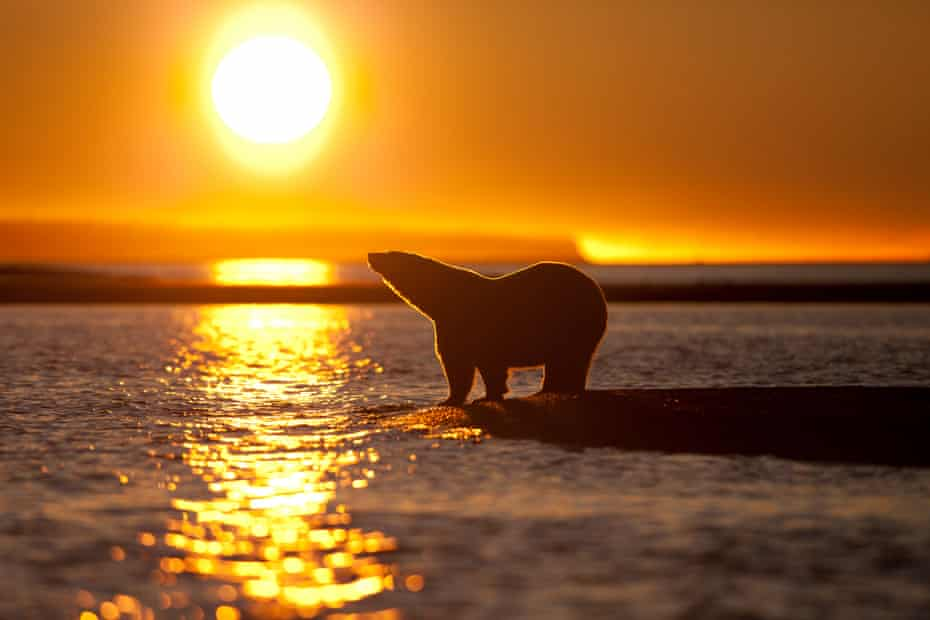
\includegraphics[scale=0.45]{graphic/polar bear.jpg}
    \caption{Polar bears have to change their behaviour to survive}
\end{figure}

Sweating, headaches, fatigue, dehydration – the ways heat exhaustion affects the human body are well documented. As temperatures inch up year by year we need to change the way we live, creating cooler places that provide refuge from heat.

But what about wildlife? We know mass die-offs are becoming more common as heatwaves sweep terrestrial and marine ecosystems, but incremental increases in temperature, which are much harder to study, are harming almost all populations on our planet.

\newpage
\begin{wrapfigure}[15]{h}{0.5\textwidth}
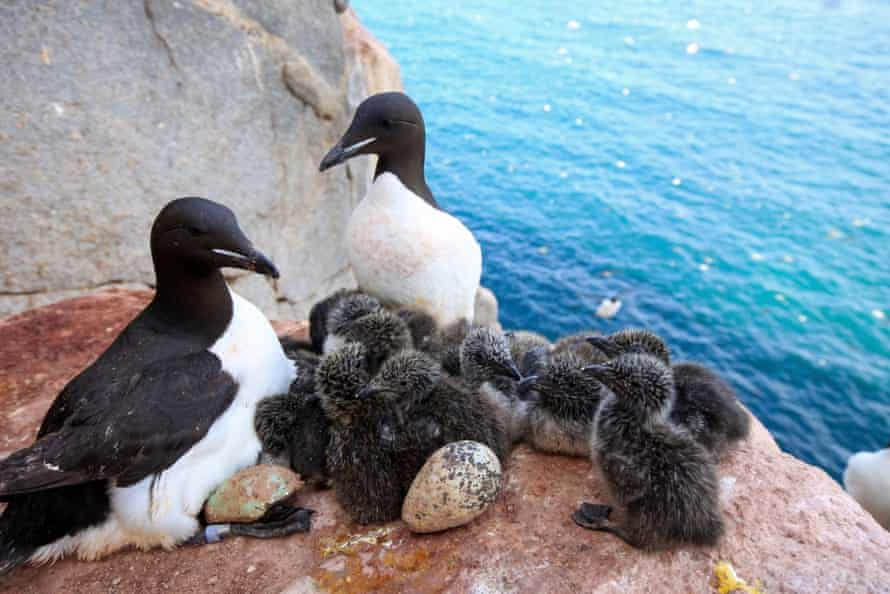
\includegraphics[scale=0.25]{graphic/seabirds.jpg}
\caption{Thick-billed murres on Coast Island in Hudson Bay, Canada}
\end{wrapfigure}
Earlier this year, for the first time, a paper was published on the impact of heat stress in large Arctic seabirds. Normally, research on species in that corner of the world is about adaptations to the cold, but in an era of climate chaos, learning to live with heat is the new challenge.

As well as undergoing physical changes, animals across the world are changing their behaviour – murres, for example, are spending more time getting into the water to cool off, leaving their eggs exposed to gulls and Arctic foxes. For parents, it’s a trade-off between keeping cool enough to avoid heat stress and protecting their young.

Many birds with similar ecological niches are at risk. Endangered bank cormorants risk overheating when sitting on eggs on exposed, rocky cliffs in southern Africa, according to research published in Conservation Physiology.

\begin{figure}[h]
\begin{minipage}{0.4\textwidth}
\centering
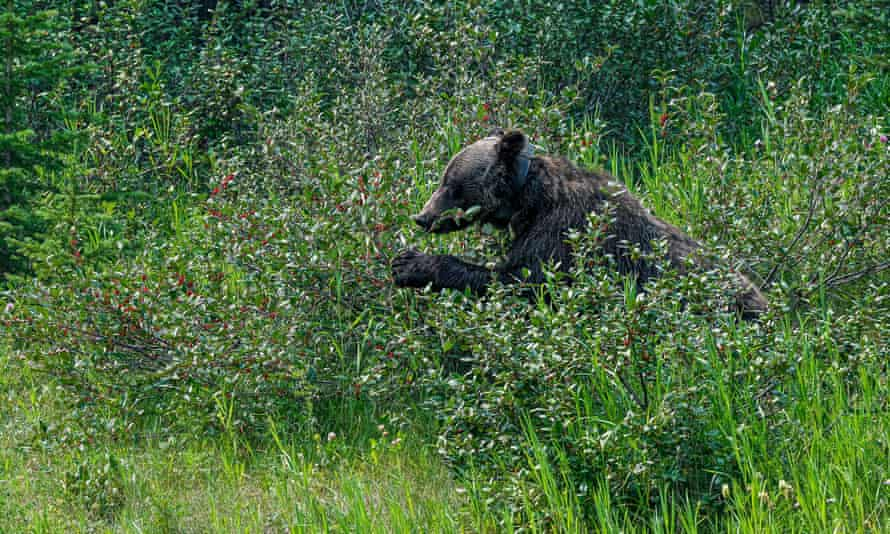
\includegraphics[scale=0.25]{graphic/bear.jpg}
\caption{Grizzly bears in Alberta, Canada}
\end{minipage}
\hfill
\begin{minipage}{0.45\textwidth}
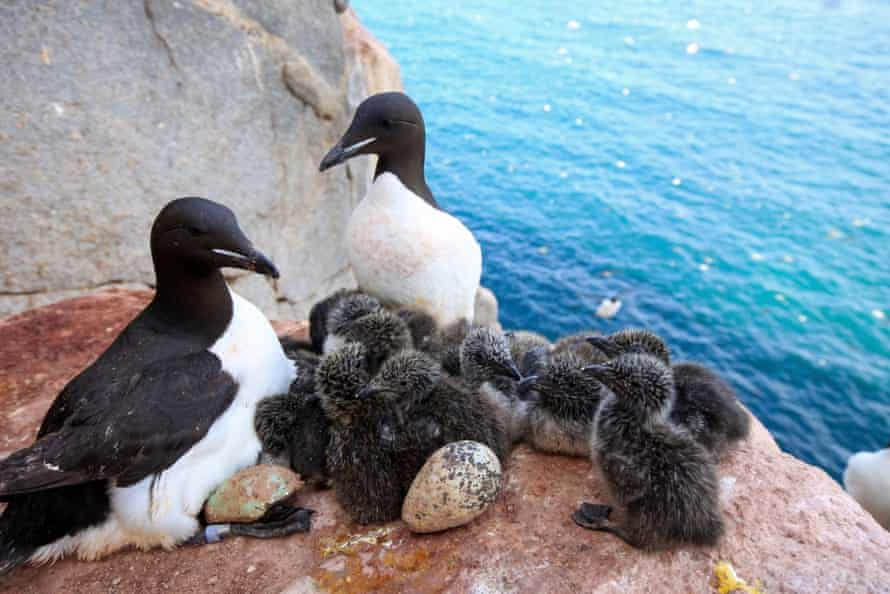
\includegraphics[scale=0.25]{graphic/seabirds.jpg}
\caption{Thick-billed murres on Coast Island in Hudson Bay, Canada}
\end{minipage}
\end{figure}
\end{document}